\documentclass[titlepage]{article}
\usepackage{graphicx}

\begin{document}

\title{Experiment 0 Lab Report}
\author{Tian Ye}

\maketitle

\begin{abstract}
Experiment 0 centers about recording an output voltage that is proportional to the force applied to the sensor by masses that are hung on its hook. The objective of said experiment is to use linear regression to find a line that most accurately reflects the data collected.
	However, there is associated uncertainty with the value of the data points collected, specifically the voltage, as we can assume that the sensor used has neither perfect accuracy nor calibration. As the recorded data will inherently have some scatter, there are many different lines with slightly different slopes and intercepts that can be considered to accurately reflect the data.
	Thus, the data analysis tool of Microsoft Excel will be used to calculate the uncertainties inherent in the slope and intercept values of the linear fit line.
\end{abstract}

\section{Data Analysis}
Before being able to perform linear regression, we first had to obtain data using various masses and their correlating voltages. As the masses are given values, there is no uncertainty regarding their measurements. The uncertainty rather instead exists in the values obtained for voltage. Below is a table illustrating the masses and the corresponding voltages reflected in the force sensor:

\begin{table}[!htbp]
\renewcommand{\arraystretch}{1.3}
\centering
\begin{tabular}{c|c|c}
    \hline
    \hline
    Mass of Weight  &  Force of Weight  &  Measured Voltage of Force Sensor\\
    \hline
    \hline

    50 grams   &   0.49 N  &  -0.08 volts\\
    \hline

    100 grams    &   0.98 N  &  -0.16 volts\\
    \hline

    200 grams  &  1.96 N  &  -0.31 volts\\
    \hline

    250 grams  &  2.45 N  &  -0.39 volts\\
    \hline

    300 grams  &  2.94 N  &  -0.46 volts\\
    \hline
\end{tabular}
\caption{Mass of Weights with the Corresponding Voltages Displayed by Force Sensor. The sensor was zeroed after every test; the 250 gram and 300 gram masses were obtained by combining the 200 gram mass with a 50 gram and 100 gram mass, respectively. Force was obtained via multiplying the mass of each weight by the gravitational constant 9.8 m/{s}$^2$.}
\label{tab:1}
\end{table}

It is important to note that the values for the table are not completely accurate as the instrument used for measuring voltage is accurate only to a certain extent; consequently, there exists uncertainty for the values of the measured voltage.
When the points in the data table are plotted on a scatterplot with the x-axis representing force in newtons and the y-axis representing the measured voltage, the following plot is created:

\begin{figure}[!htbp]
    \centering
    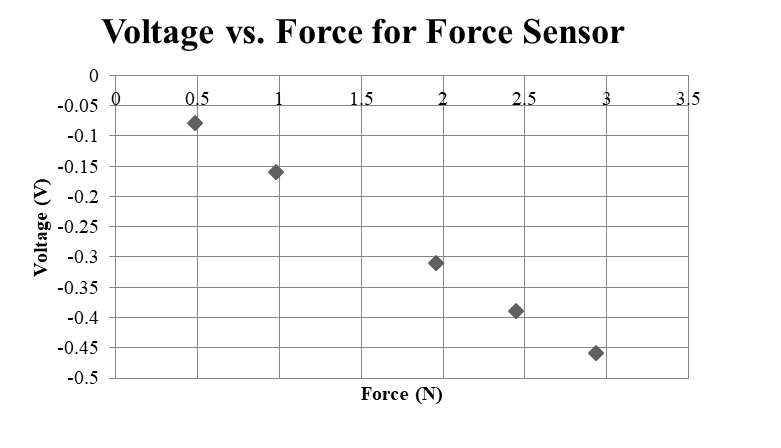
\includegraphics[width=3.0in]{Scatterplot.png}
    \caption{Voltage (V) displayed on Force Sensor plotted against Force (N). The data points follow a relatively linear progression. The data points were collected from left to right with: 50 gram mass, 100 gram mass, 200 gram mass, 200 + 50 gram mass, 200 + 100 gram mass.}
    \label{fig:1}
\end{figure}

Given these points, we can now begin to solve for the linear fit line. The line will be presented in the form of the equation below:

\begin{equation}
    \label{eq:line_regres}
    V = aF+b
\end{equation}

The equation of the linear fit line calculated by Microsoft Excel is

\begin{equation}
    \label{eq:line_fit}
     V = -0.1554F - 0.0058
\end{equation}

However, this equation has uncertainty factored in for neither \textit{a} nor \textit{b}. The scatterplot with the linear fit line is displayed below:

\begin{figure}[!htbp]
    \centering
    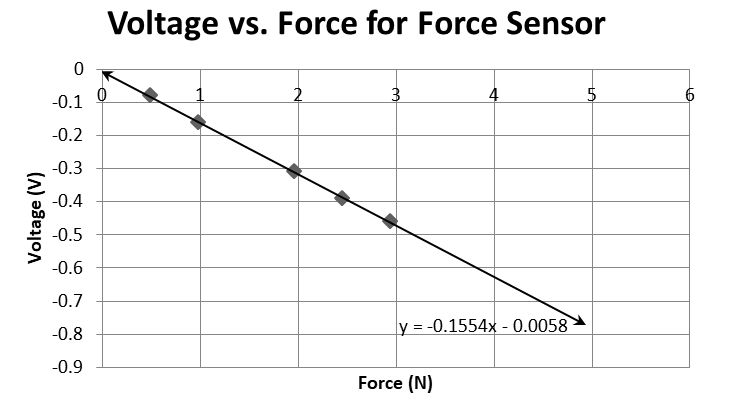
\includegraphics[width=3.0in]{LinReg.png}
    \caption{Voltage (V) displayed on Force Sensor plotted against Force (N) with linear fit line, as generated by Microsoft Excel.}
    \label{fig:2}
\end{figure}

To solve for $\delta$\textit{a} and $\delta$\textit{b}, the Regression tool was used  in Microsoft Excel. From the Regression tool, we obtain the following values for Standard Error:

\begin{center}
$\delta$\textit{a} = 0.00146924344415493 V/N
\end{center}

\begin{center}
$\delta$\textit{b} = 0.00291549140606069 V
\end{center}

However, the precision of both $\delta$\textit{a} and $\delta$\textit{b} is much higher than what the uncertainty would indicate. Consequently, the only value that will be kept is the first nonzero digit for both $\delta$\textit{a} and $\delta$\textit{b}:

\begin{center}
$\delta$\textit{a} = 0.001 V/N
\end{center}

\begin{center}
$\delta$\textit{b} = 0.003 V
\end{center}

This in turn will lead us to the final equation of the linear fit line:

\begin{equation}
    \label{eq:line_fit}
     V = aF - b
\end{equation}

\begin{center}
\textit{a} = -0.1554 $\pm$ 0.001 V/N
\end{center}

\begin{center}
\textit{b} = -0.0058 $\pm$ 0.003 V
\end{center}

With \textit{a} and \textit{b} having blank significant figures each.

\section {Conclusion}
The goal of Experiment 0 was to provide insight into the lab report writing process via the task of finding a linear fit line for data collected via a force sensor. The result demonstrated that while the linear regression tool can provide a relatively precise linear fit line for the given data, there nonetheless exists uncertainty regarding both the \textit{a} and \textit{b} values within the equation. The most lilkely cause of error in this experiment then can be attributed to inaccuracies of measurement, specifically the fact that the force sensor cannot be infinitely precise. This henceforth created some spread in the data, which is then reflected in the fact that there is not a perfect linear fit line but rather several applicable ones. This fact is then reflected in the $\delta$\textit{a} and $\delta$\textit{b} values in the final equation.

\end{document}
T